\documentclass{article}
\usepackage[utf8]{inputenc}
\usepackage[spanish, es-tabla]{babel}
\usepackage{amsmath}
\usepackage{amsfonts}
\usepackage{siunitx}
\usepackage{amssymb}
\usepackage{graphics}
\usepackage{float}
\usepackage{lipsum}
\usepackage{multicol}
\usepackage{graphicx}
\usepackage{multirow}
\usepackage{wrapfig}
\usepackage{subcaption}
\usepackage[hidelinks]{hyperref}
\usepackage{enumitem}
\usepackage{graphicx}
\usepackage{mwe}
\usepackage{lipsum}
\usepackage{caption}
\usepackage{booktabs}
\usepackage{textcomp, gensymb}

%-------Márgenes--------
\usepackage{geometry}
\newgeometry{
    left=2.54cm,
    right=2.54cm,
    top=2.4cm,
    bottom=2.4cm}
%-------Pie de Página--------
\usepackage{fancyhdr}
\pagestyle{fancy}
\fancyhf{}    % Quitar configuración por defecto
\renewcommand{\headrulewidth}{0pt}  %Quitar linea del encabezado
\cfoot[]{}   
\lfoot[]{\small \textit{Termodinámica modulo experimental, 2023} }
\rfoot[]{\textit{\thepage}}
\setcounter{page}{1}   %Numeración
%\usepackage{showframe}
%--------------------------------------------------------------



\date{}
%===============================================================
% Inicio del documento
\begin{document}
 
     \begin{center}
    % TÍTULO DEL TRABAJO
        {\Large \textbf{Ley de enfriamiento de Newton}}\\
        \vspace{5mm}
        % AUTORES 
        {\small \textbf{A.F.Suarez Reyes $^{1}$},\textbf{J.S. Palacio Correa$^{2}$},\textbf{M. García Mejía$^{3}$} \\
        \vspace{3mm}}
        % AUTORES 
        {\small \textit{Departamento de Física, Universidad Nacional de Colombia, Sede Bogotá, Bogotá, Colombia.}}\\
        \vspace{3mm}
        % FECHA 
        {\small 02/10/2023}\\
        \vspace{3mm}
        {\texttt{\textup{asuarezre@unal.edu.co$^{1}$, jspalacioco@unal.edu.co$^2$, mgarciamej@unal.edu.co$^{3}$}}} \\
    \end{center}
    
    
    \vspace{5mm}

% RESUMEN
{\large \textbf{Resumen}}\\
aaaaa


\textit{ \hspace{2mm}}


\section{Introducción}

En un sistema donde los cuerpos presentan diferencias en sus temperaturas habrá un intercambio de energía hasta que el sistema alcance el equilibrio. A esta transferencia de energía  se le conoce como calor y puede presentarse por convección, radiación o conducción. 
En nuestro sistema colocamos varios elementos en contacto con el medio ambiente después de aumentar su temperatura . Una ley que nos permite modelar la transferencia de calor en esta experiencia es la conocida ley de enfriamiento de Newton, la cual establece que: 

\begin{align}
    \frac{dQ}{dt} = hA_s(T_s-T_A) 
\end{align}

donde,  \\ 
$h$:  Coeficiente de transmisión o conductancia térmica  \\ 
$A_s$: Área superficial del cuerpo en contacto con el fluido \\ 
$T_s$: Temperatura en la superficie del cuerpo \\ 
$T_A$: Temperatura del medio ambiente

Las perdidas de calor experimentadas por el cuerpo de mayor temperatura son proporcionales a la diferencia de temperatura y son expresadas por la siguiente relación 

\begin{align}
    dQ = -mc_edT
\end{align}

donde, \\ 
$m$: Masa del cuerpo \\ 
$c$: calor especifico \\ 
De las ecuaciones(1) y (2) obtenemos la siguiente expresión para la ley de enfriamiento de Newton 

\begin{align}
    \frac{dT}{dt} = -k(T-T_A)
\end{align}

$k$ es una constante de proporcionalidad conocida como parámetro de enfriamiento.

\begin{align}
    k = \frac{hA_s}{mC_e}
\end{align}

La solución a la ecuación diferencial (3) es: 

\begin{align}
    T(t) = T_A + Ce^{-\frac{t}{\tau}}
\end{align}

$\tau = k^{-1}$ representa el tiempo característico de enfriamiento \\ 

Asumiendo una temperatura inicial $T_i$, obtenemos: 

\begin{align}
    T(t) = T_A + (T_i-T_f)e^{-\frac{t}{\tau}}
\end{align}

En el caso donde el sistema presente una fuente de energía que le proporcione calor, la energía suministrada la podemos expresar como: 

\begin{align}
    P = mc\frac{dT}{dt}
\end{align}

De donde obtenemos la siguiente expresión lineal para la temperatura: 

\begin{align}
    T =  T_A + \frac{P}{mc}t
\end{align}

Si en el sistema existen perdidas por convección el balance de energía debe expresarse de la siguiente manera: 

\begin{align}
    P = mc \frac{dT}{dt} + hA(T-T_A) \\ 
    \frac{dT}{dt} = \frac{P}{mc} - \frac{hA}{mc}(T-T_A)
\end{align}

La solución de esta ecuación para un sistema que recibe calor de una fuente externa(fuente de voltaje) y además esta afectado por la ley de enfriamiento de Newton, variando desde la temperatura ambiente $T_A$ hasta una temperatura $T$

\begin{align}
    T = T_A +\frac{P}{hA}[1-e^{-\frac{hA}{mc}t}]
\end{align}


\section{Desarrollo experimental}

El objetivo de esta practica es comprobar la validez de la ley de enfriamiento de Newton[ecuación(6)]. Con este objetivo en mente la practica consistió en dos partes, la primera en elevar la temperatura de 5 cilindros de (hierro o acero????)  y permitir que estos se enfriaran a temperatura ambiente mientras mediamos su temperatura en función del tiempo. 
Para elevar la temperatura del cilindro, este fue sumergido en agua hasta alcanzar la temperatura de ebullición( $90°$), a su vez en su interior estaba dispuesto un termopar que media la temperatura al retirarlo y dejarlo suspendido mientras interacciona con el ambiente(Aire). Durante este proceso de enfriamiento con ayuda de un multímetro pudimos registrar el cambio de temperatura hasta que esta tomara un valor mas o menos constante o variara muy poco. El anterior procedimiento se repitió para 5 cilindros con diferentes geometrías.  \\ 
La segunda parte de la practica consistió en aumentar la temperatura de un cilindro de bronce que contiene una resistencia eléctrica en su interior con ayuda de una fuente, la recolección de los datos de temperatura en función del tiempo fue exactamente igual que la primera parte.


\subsection{Materiales e instrumentos}

\begin{multicols}{2}
\begin{itemize}
    \item Multímetro
    \item Fuente eléctrica 
    \item Estufa
    \item Recipiente de agua
    \item Termopar
    \item Cilindro de bronce con medidas:
        213213
    \item 5 Cilindros de hierro/acero con medidas: 
        \begin{itemize}
        \item 1
        \item 2
        \item 3
        \item 4
        \item 5
        \end{itemize}
\end{itemize}
\end{multicols}

\subsection{Montaje}

\begin{figure}[H]
    \centering
    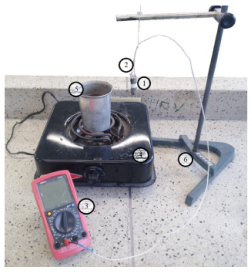
\includegraphics{media/Montaje.png}
    \caption{Montaje experimental: Ley de enfriamiento.}

    
\end{figure}


\section{Resultados y Análisis}
\subsection{Enfriamiento}
El comportamiento general de la temperatura de los cilindros al enfriarse fue la esperada de acuerdo con la ecuación XX. Al conocer de antemano los parámetros correspondientes a las temperaturas iniciales y finales del cilindro al, el ajuste se simplificó a la búsqueda única de la constante de enfriamiento $\tau$. Así, obtenemos lo siguiente:

\begin{figure}[H]
    \centering
    \begin{subfigure}[t]{0.5\textwidth}
        \centering
        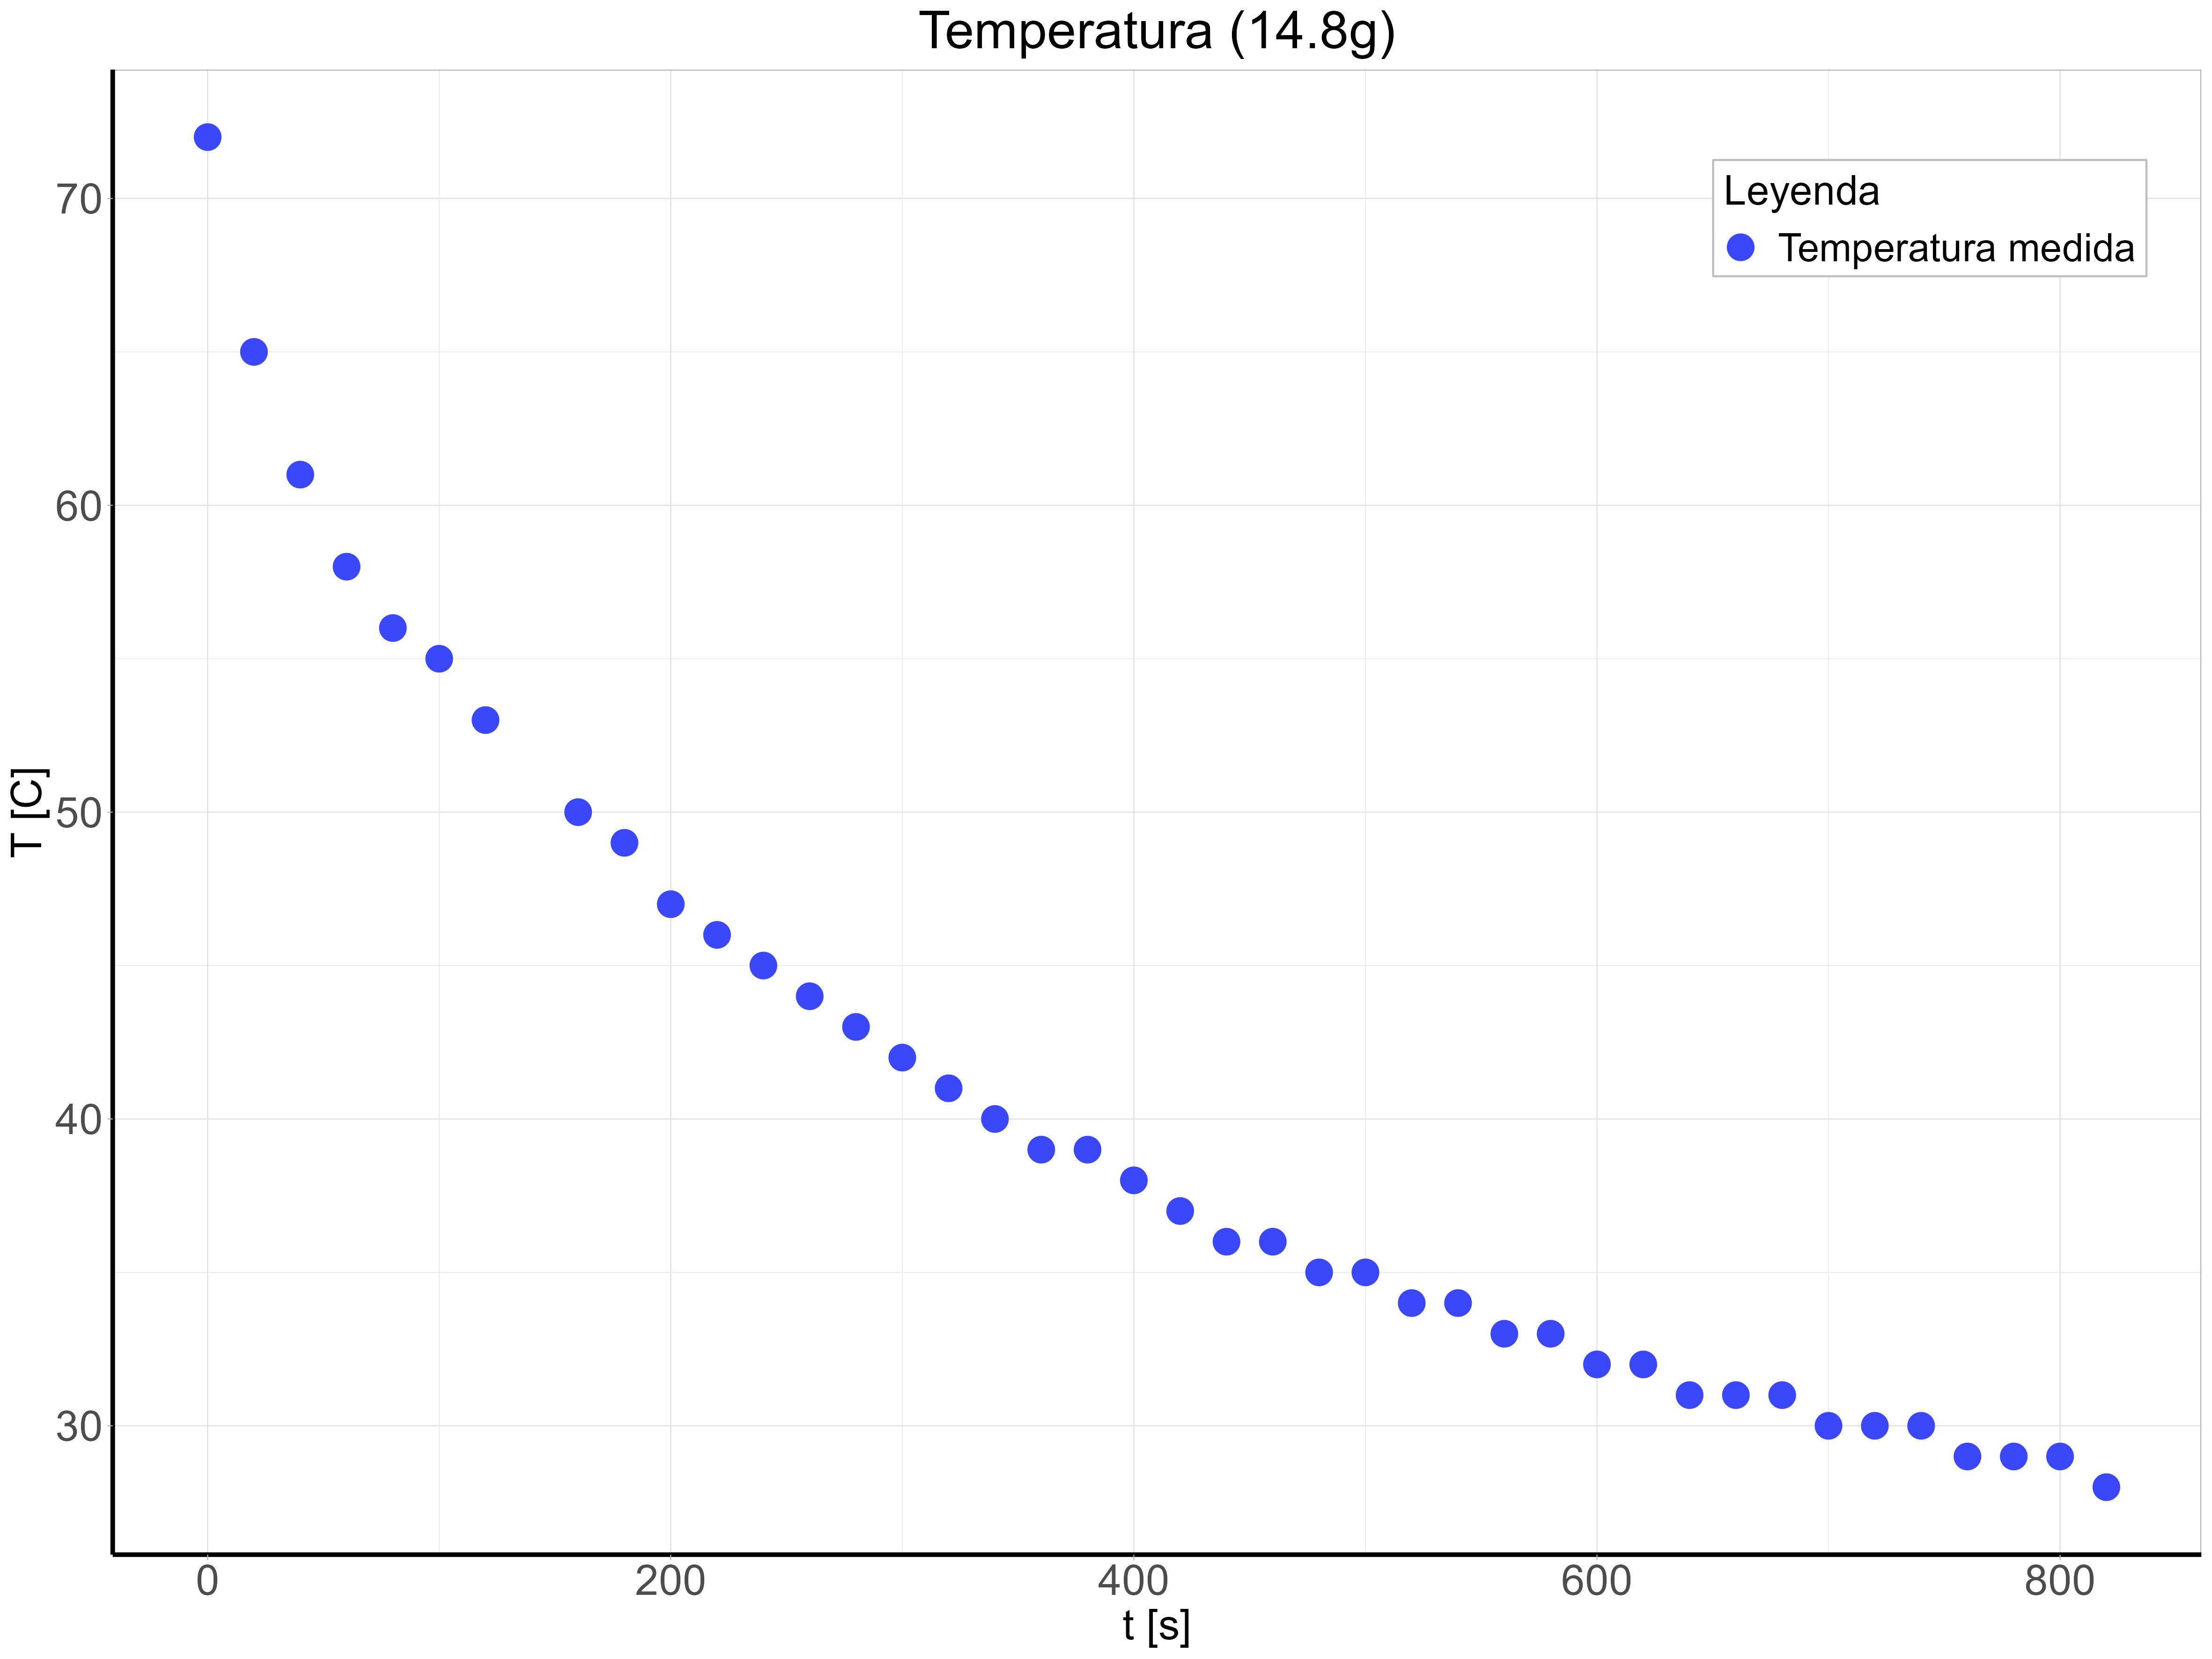
\includegraphics[height=5cm]{media/Tvt_1.png}
        \caption{Primera medición}
    \end{subfigure}%
    ~ 
    \begin{subfigure}[t]{0.5\textwidth}
        \centering
        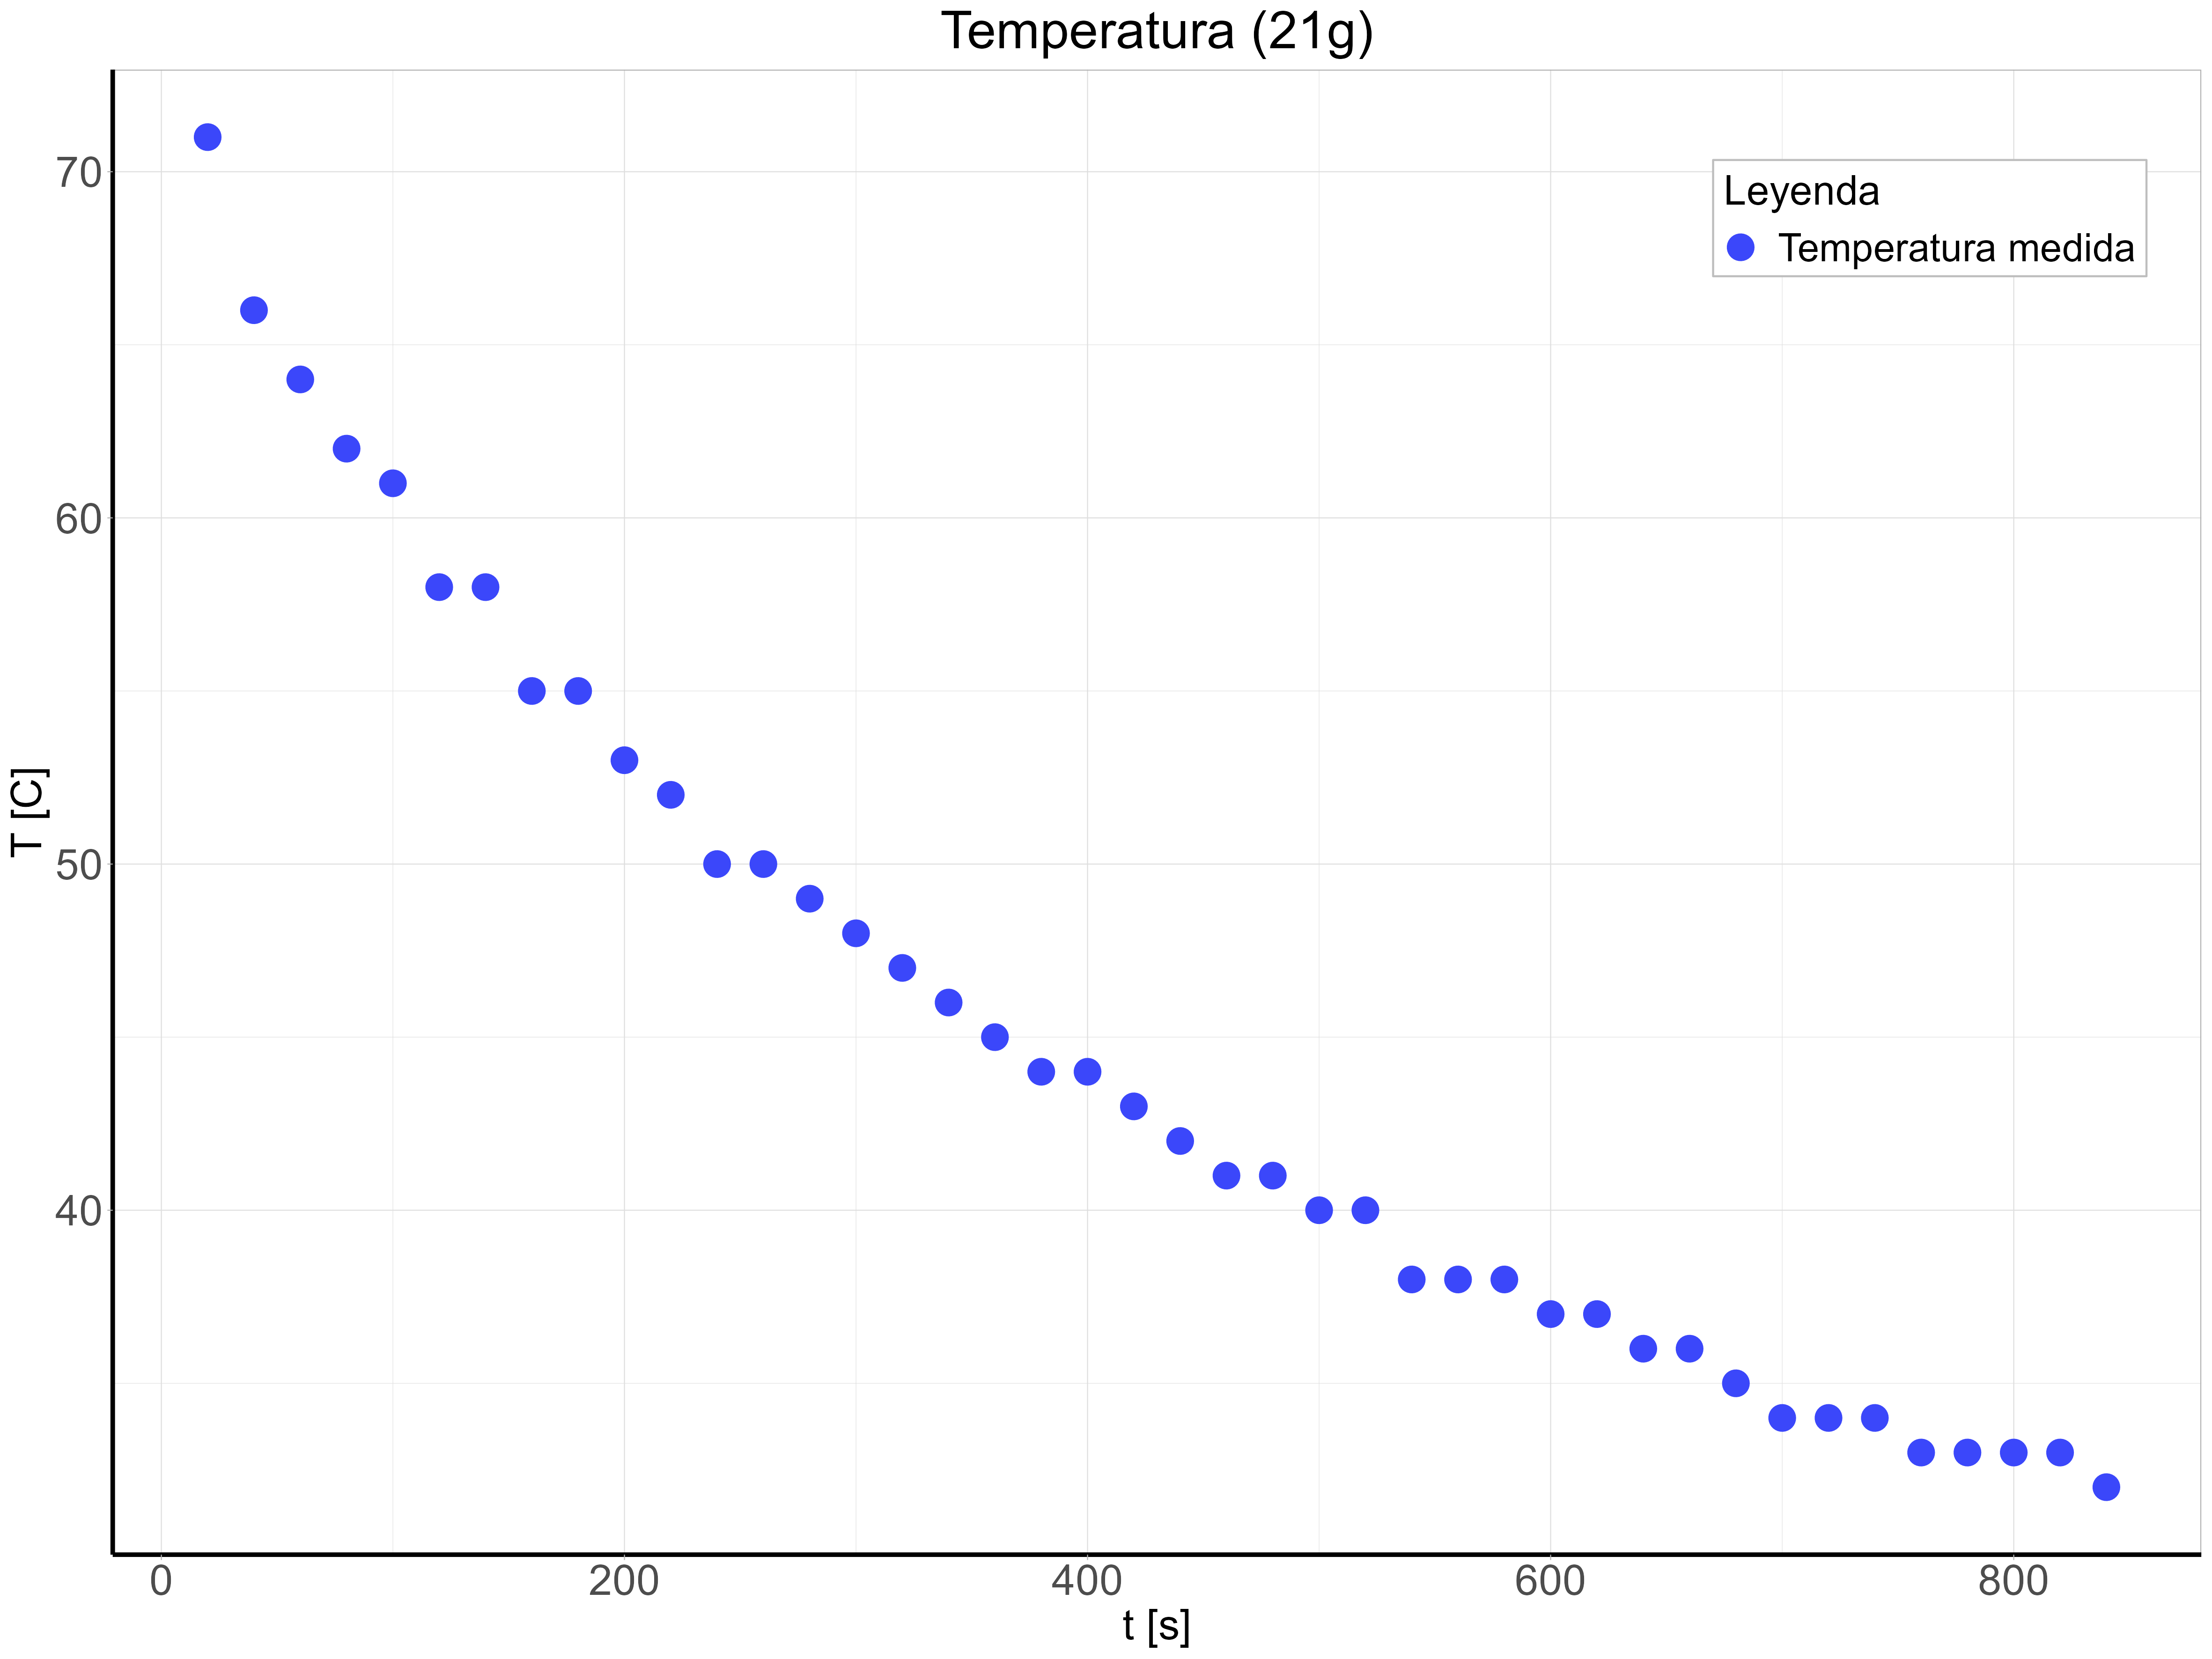
\includegraphics[height=5cm]{media/Tvt_2.png}
        \caption{Segunda medición}
    \end{subfigure}
    ~ 
    \begin{subfigure}[t]{0.5\textwidth}
        \centering
        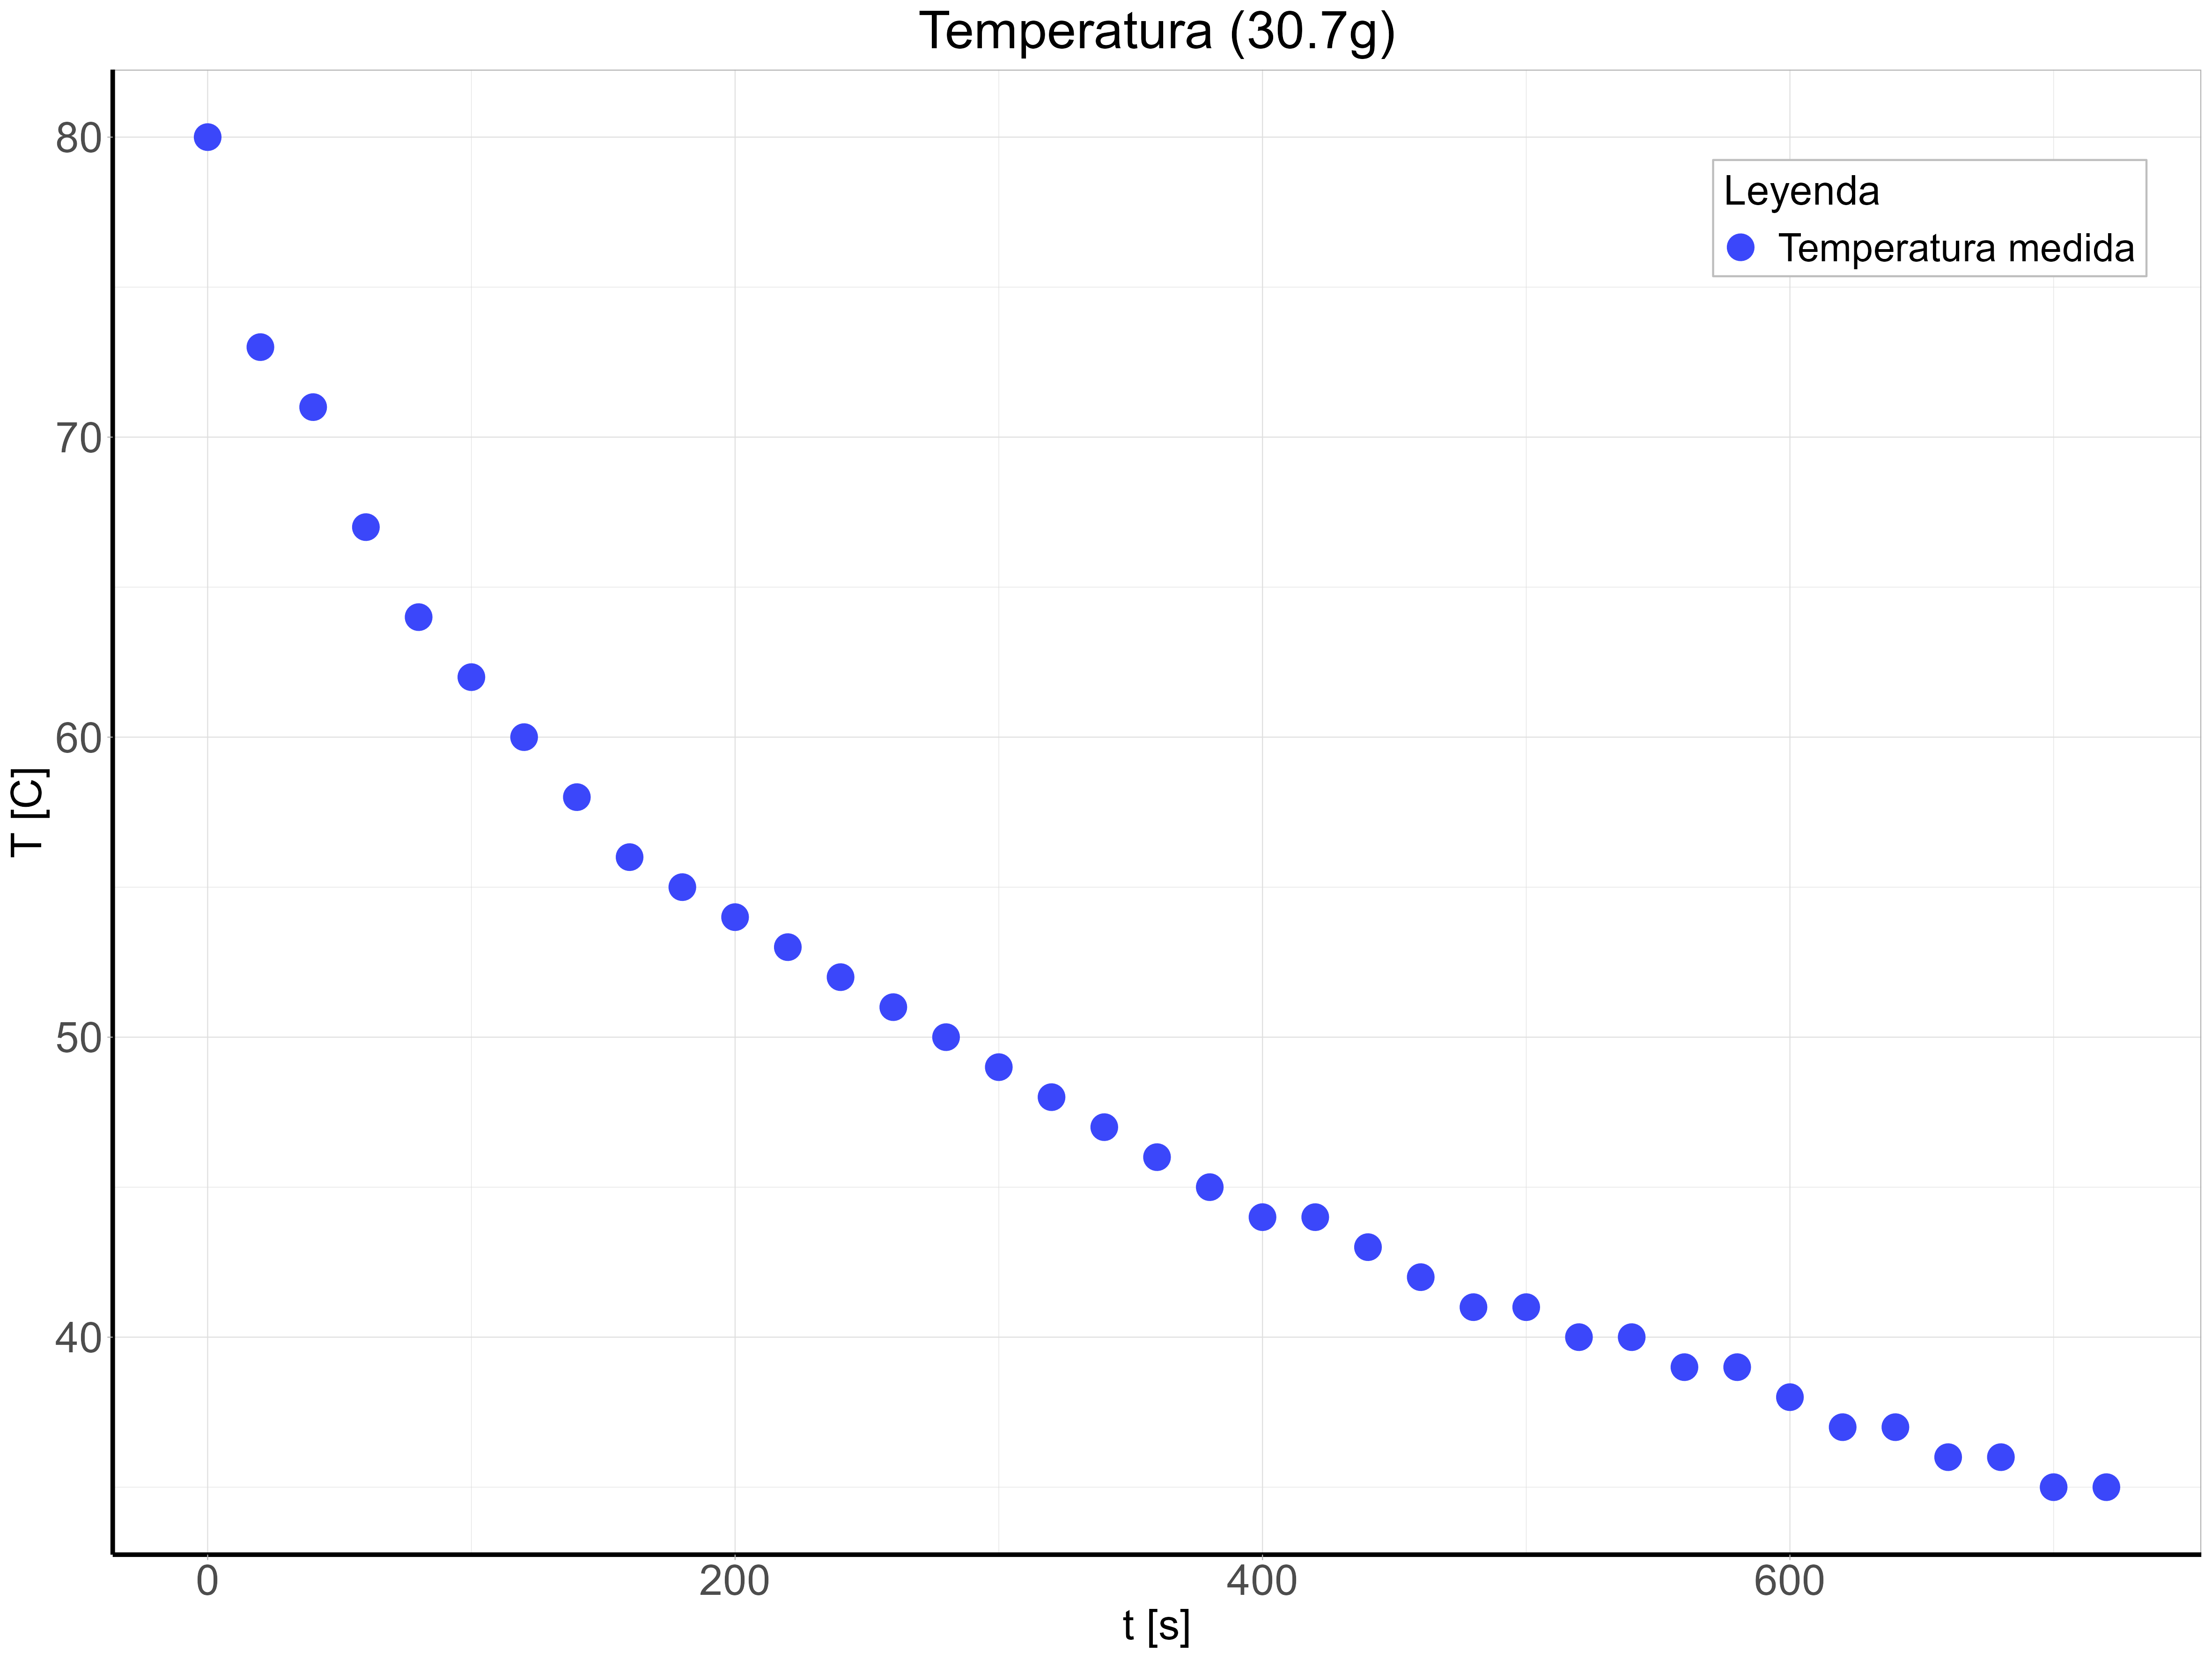
\includegraphics[height=5cm]{media/Tvt_3.png}
        \caption{Segunda medición}
    \end{subfigure}
    ~ 
    \begin{subfigure}[t]{0.5\textwidth}
        \centering
        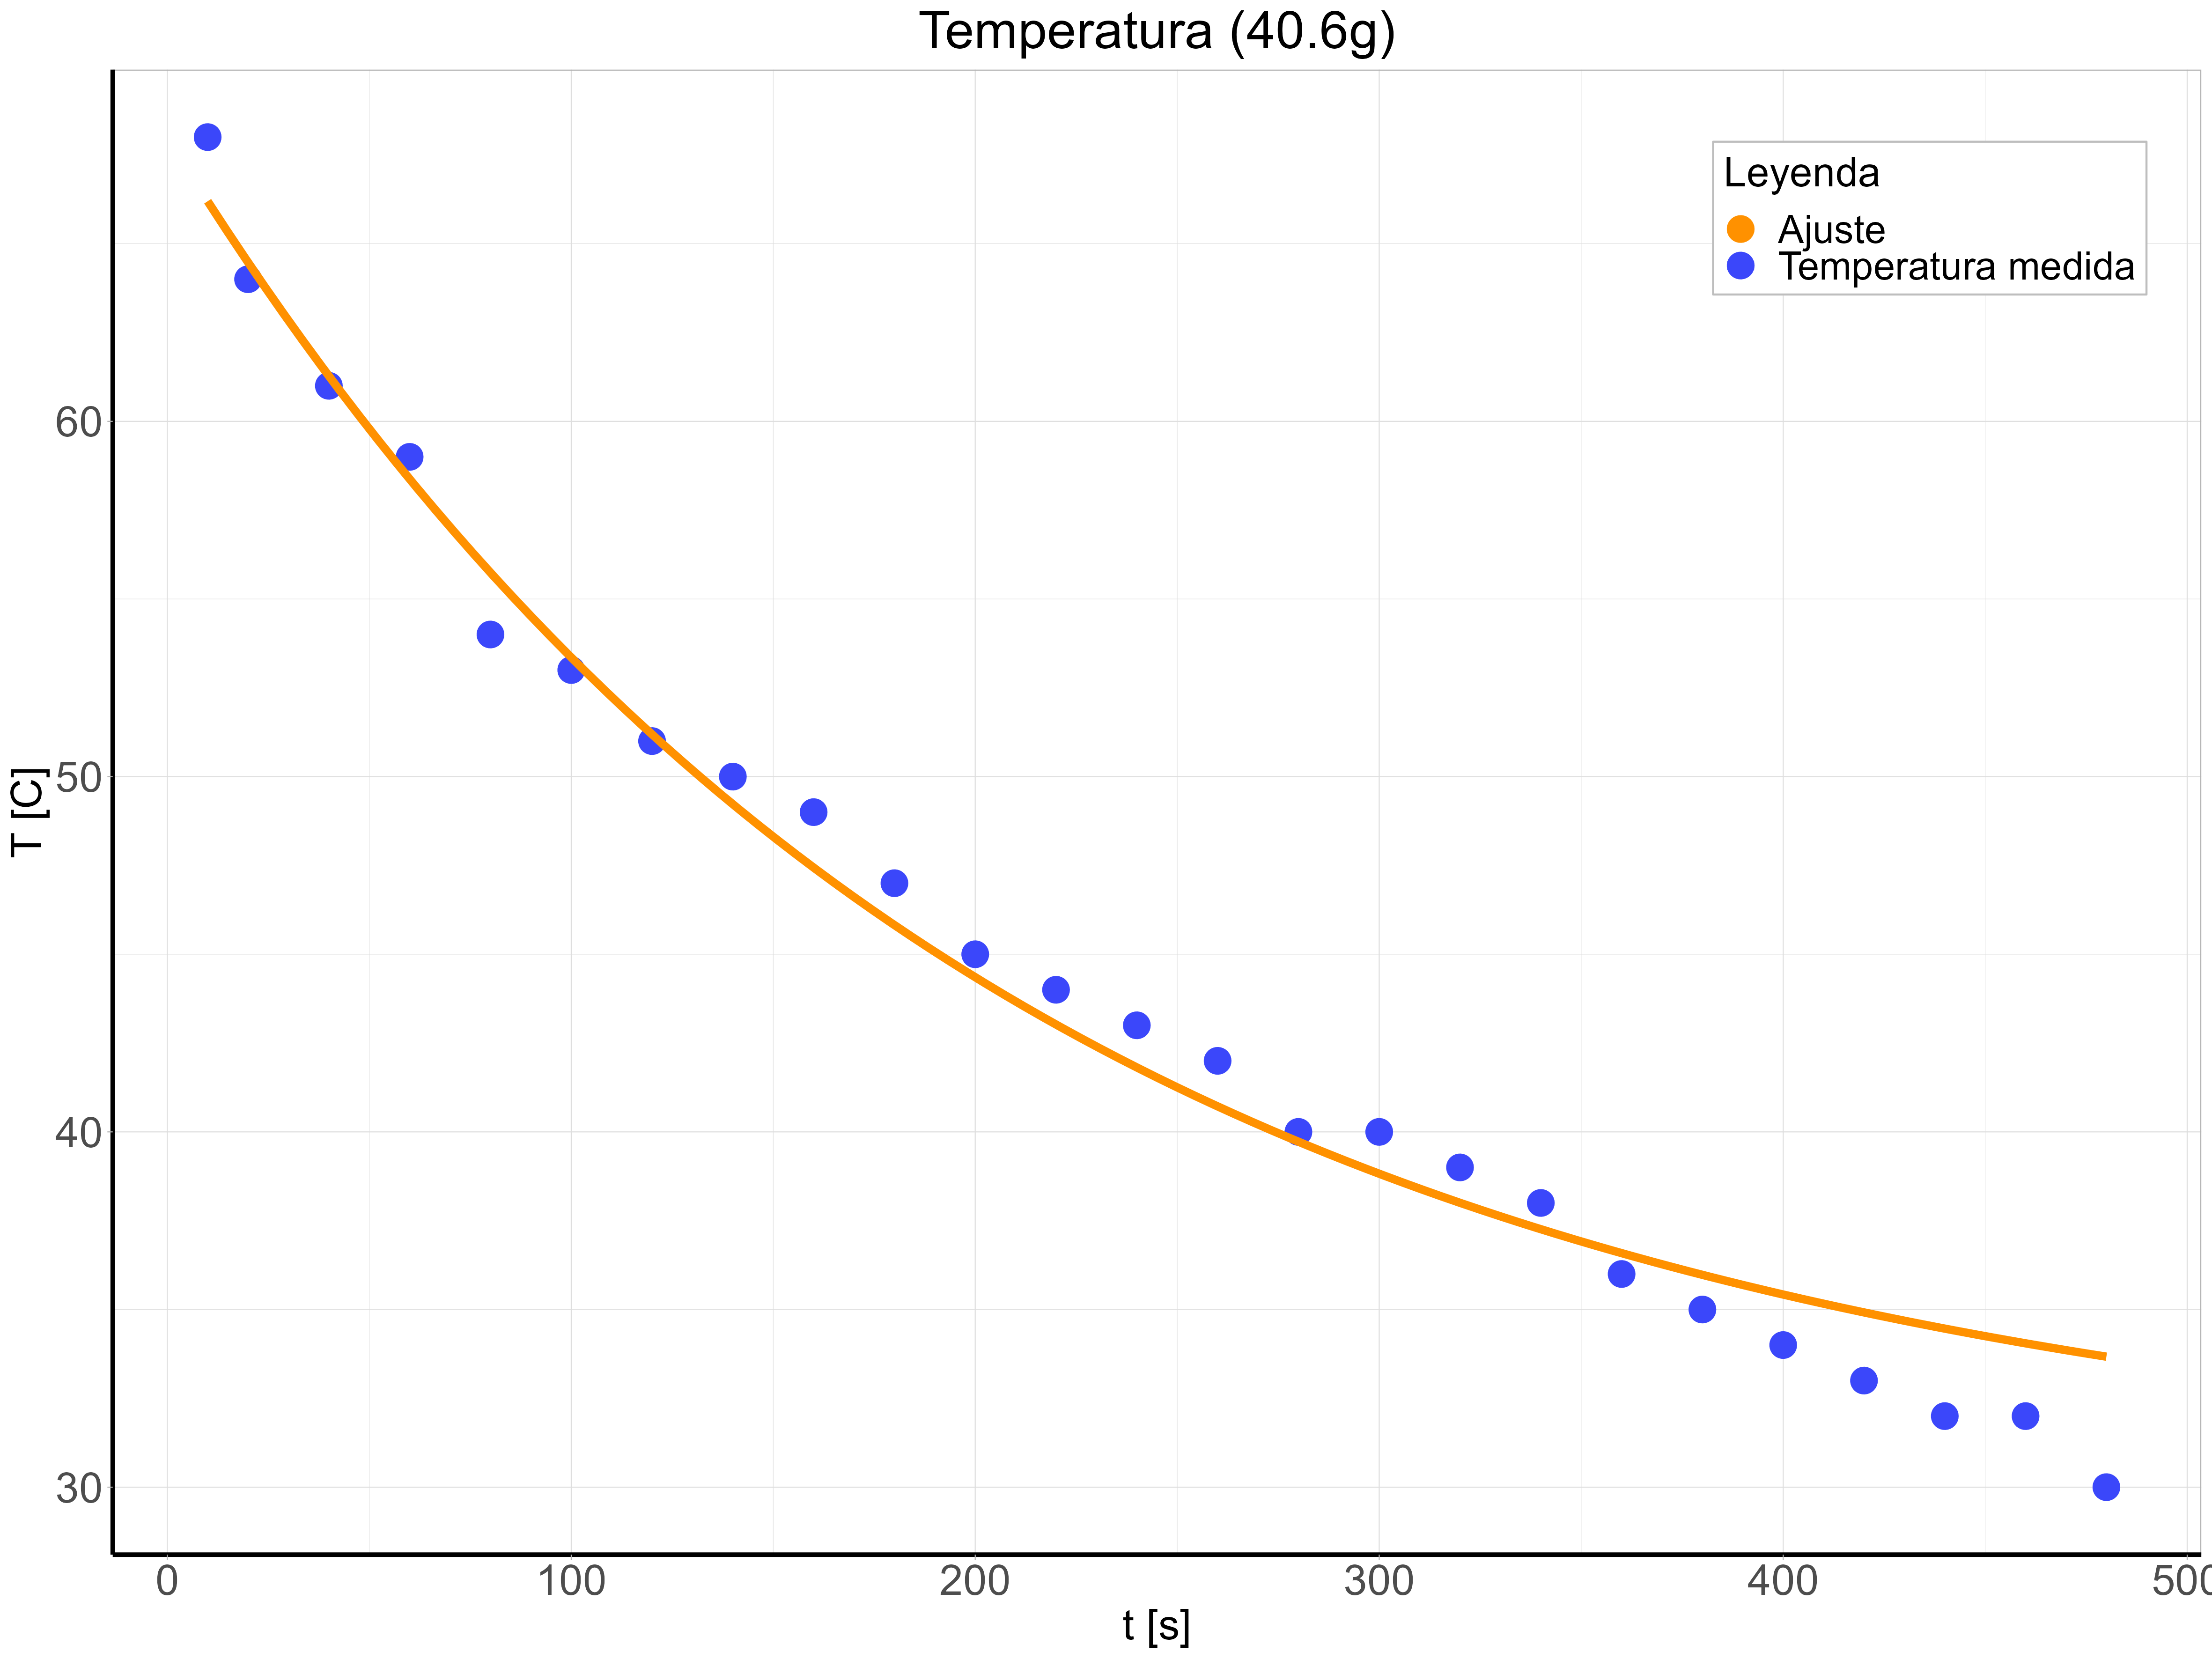
\includegraphics[height=5cm]{media/Tvt_4.png}
        \caption{Primera medición}
    \end{subfigure}%
    ~ 
    \begin{subfigure}[t]{0.5\textwidth}
        \centering
        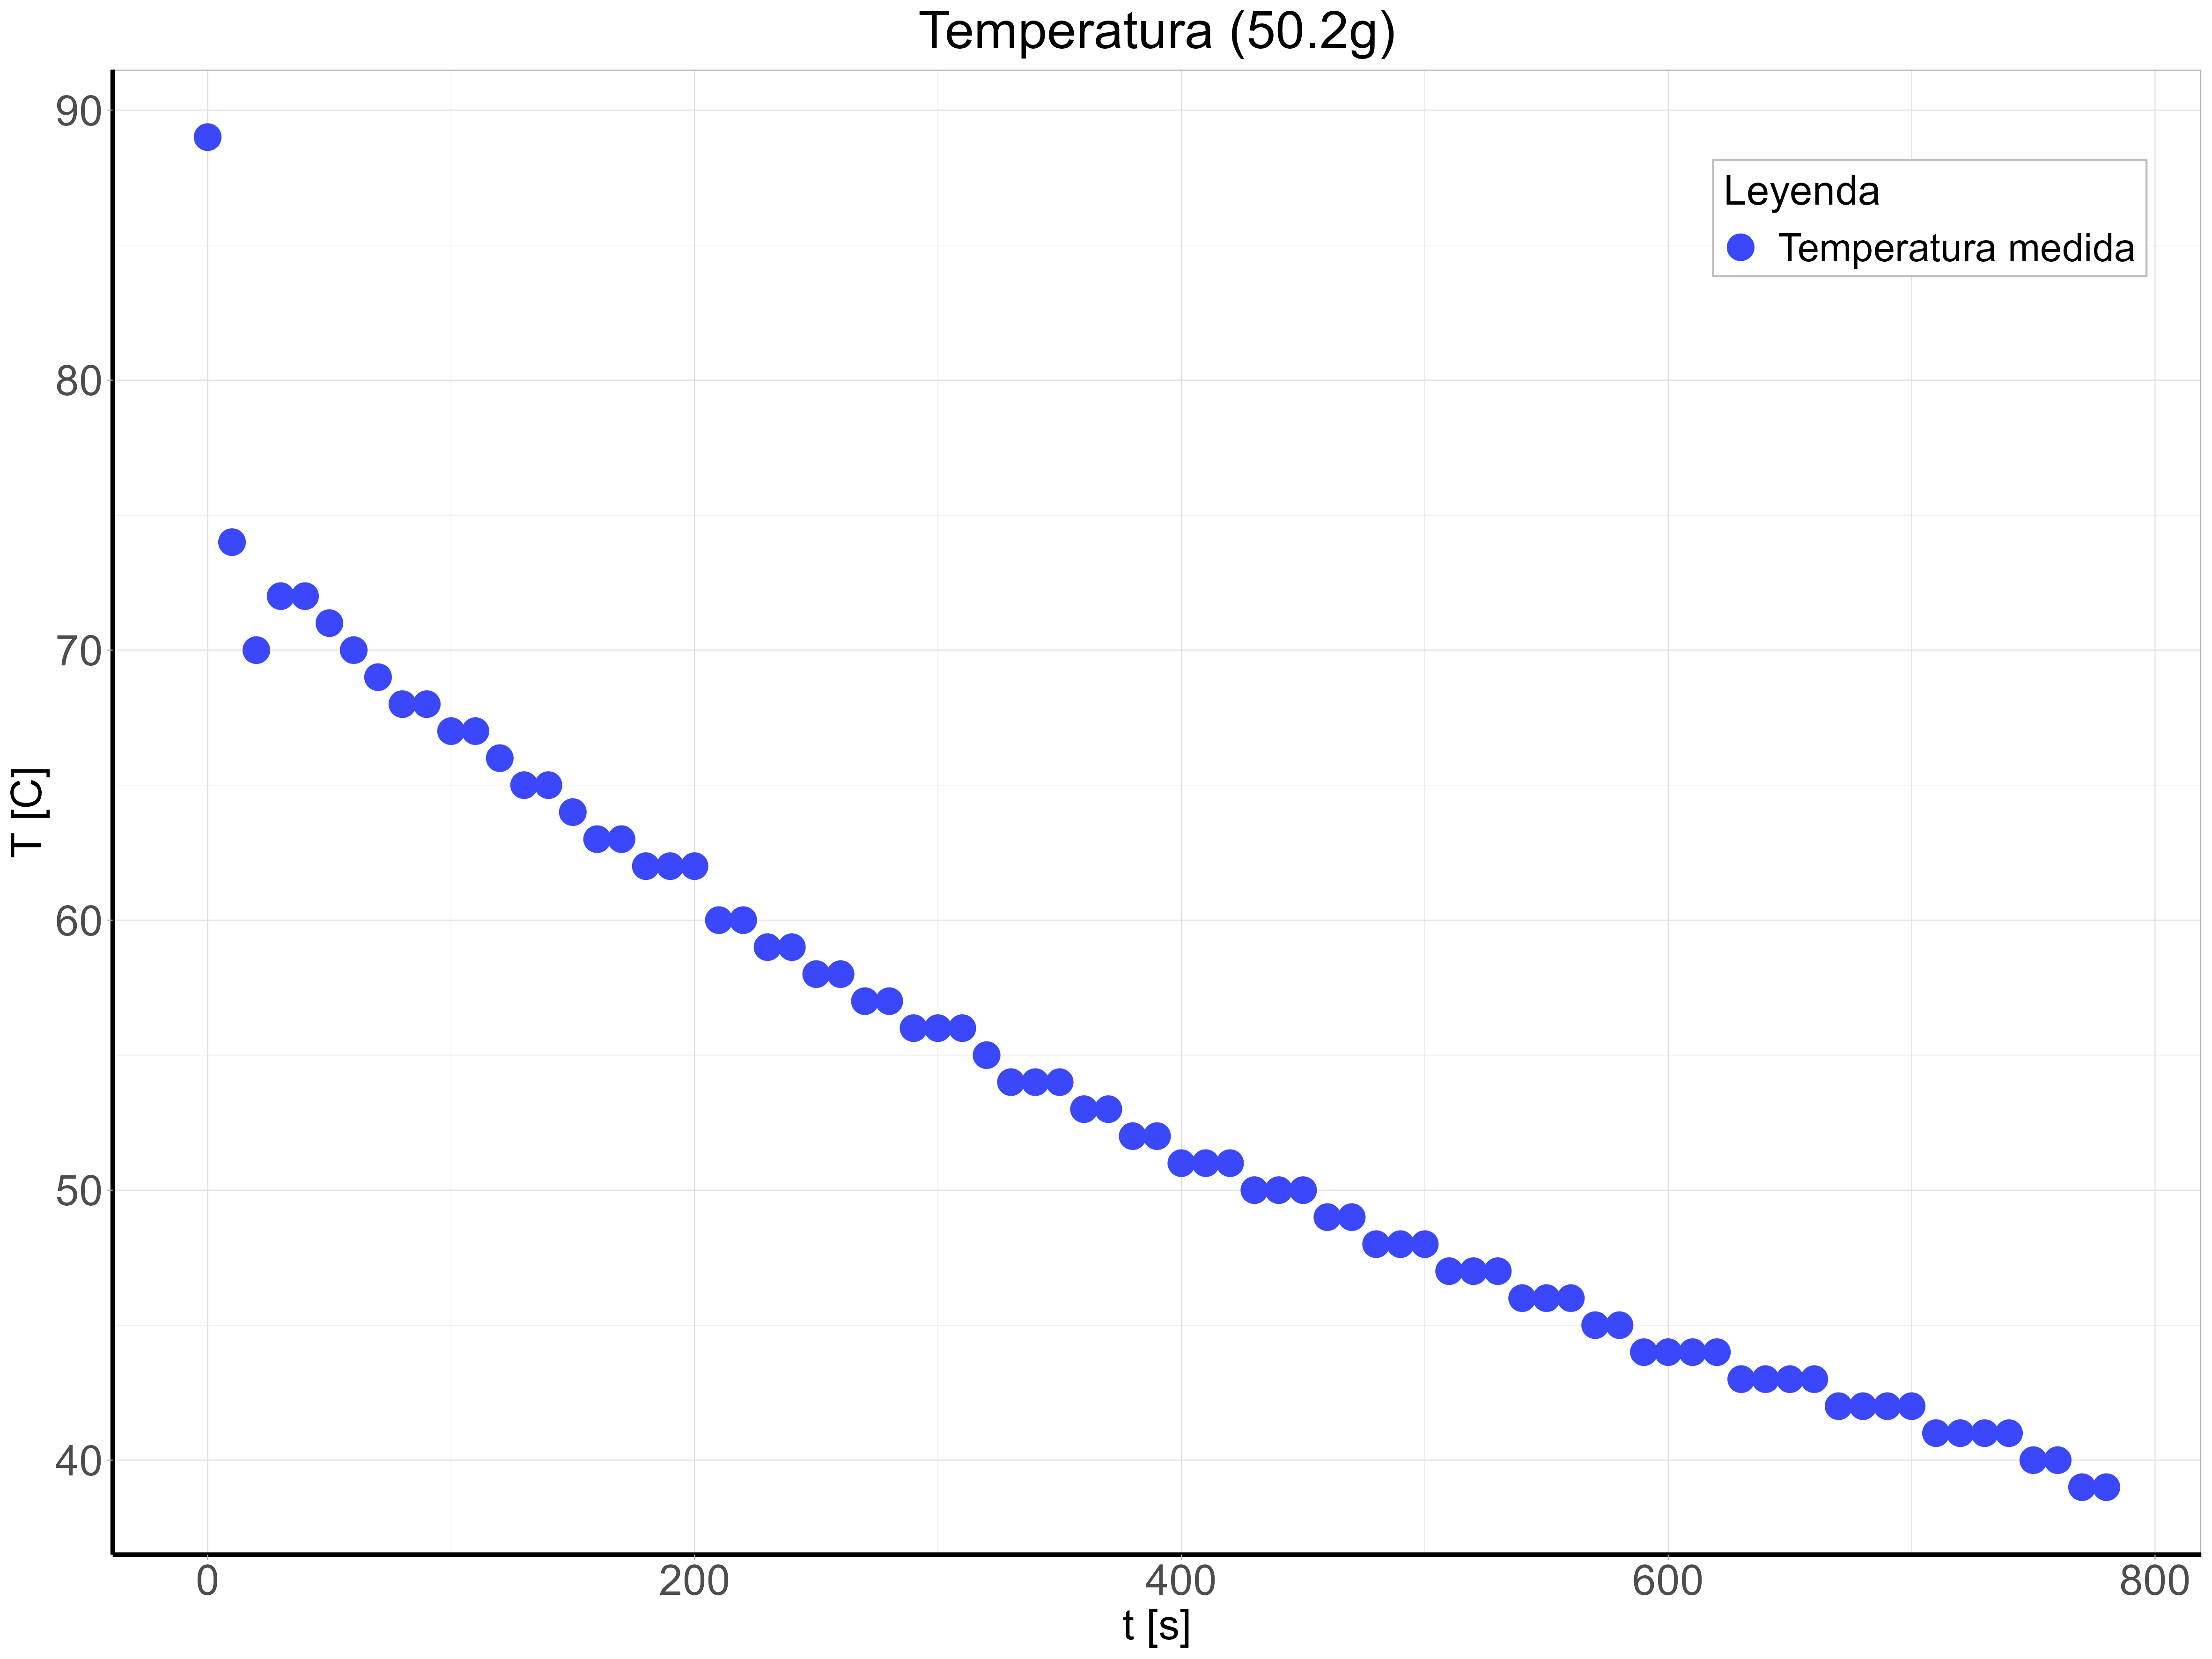
\includegraphics[height=5cm]{media/Tvt_5.png}
        \caption{Segunda medición}
    \end{subfigure}
    \caption{Aumento de la temperatura en el tiempo dentro del calorímetro.}
    \label{fig:electemp}
\end{figure}

De este modo, se encontraron los siguientes valores de la constante $\tau$:

\begin{table}[H]
    \centering
    \begin{tabular}{l|l}
    Masa     & $\tau$ $(s)$       \\
    \hline
    $14.8g$  & $(246.34 \pm 0.0)$ \\
    $21g$    & $(311.25 \pm 0.0)$ \\
    $30.7g$  & $(232.50 \pm 0.0)$ \\
    $40.6g$  & $(205.43 \pm 0.0)$ \\
    $50.2g$  & $(335.60 \pm 0.0)$ \\
    \end{tabular}
    \end{table}

Vale la pena, además, considerar cómo estas constantes se relacionan con las condiciones geométricas y físicas de los cilindros; es decir, con su área superficial y masa. Es importante aclarar de antemano que no se espera mucho diferencia entre estas dos características dada la idéntica composición de los bloques, lo que implica que el área y la masa tienen un relación proporcional directa. Veamos:

\begin{figure}[H]
    \centering
    \begin{subfigure}[t]{0.5\textwidth}
        \centering
        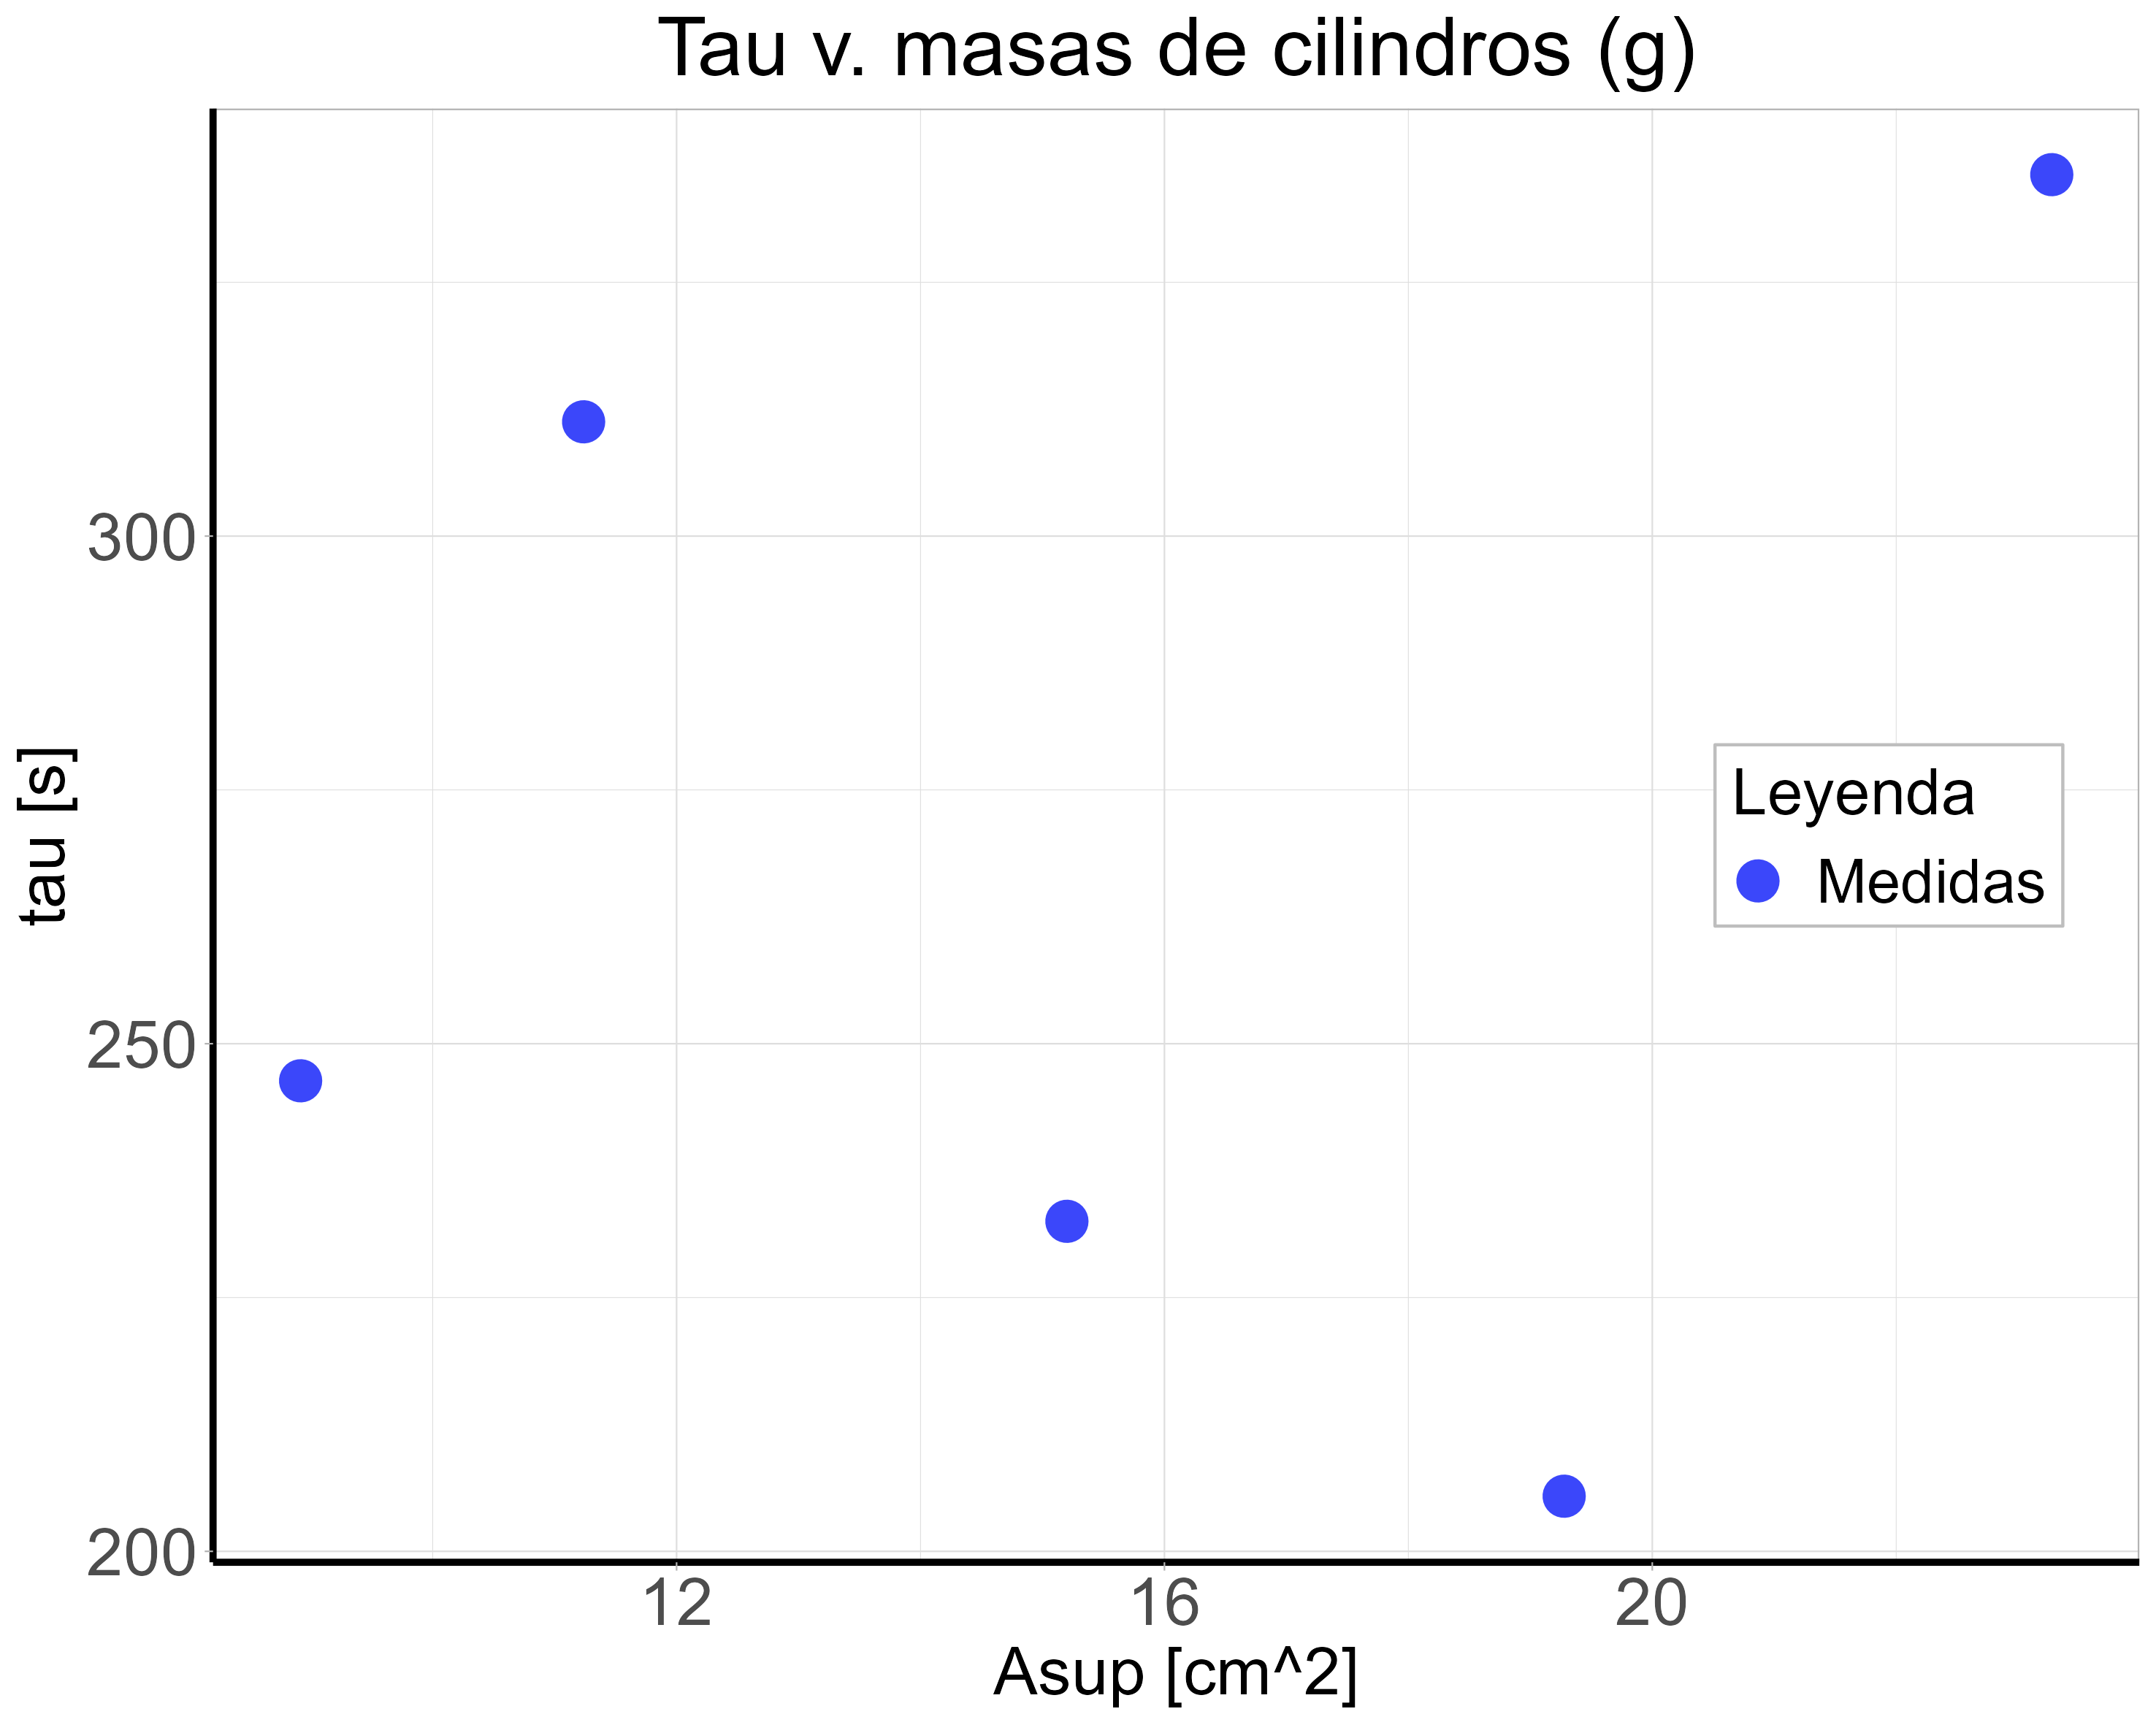
\includegraphics[height=5cm]{media/TauvAsup.png}
        \caption{Primera medición}
    \end{subfigure}%
    ~ 
    
    \begin{subfigure}[t]{0.5\textwidth}
        \centering
        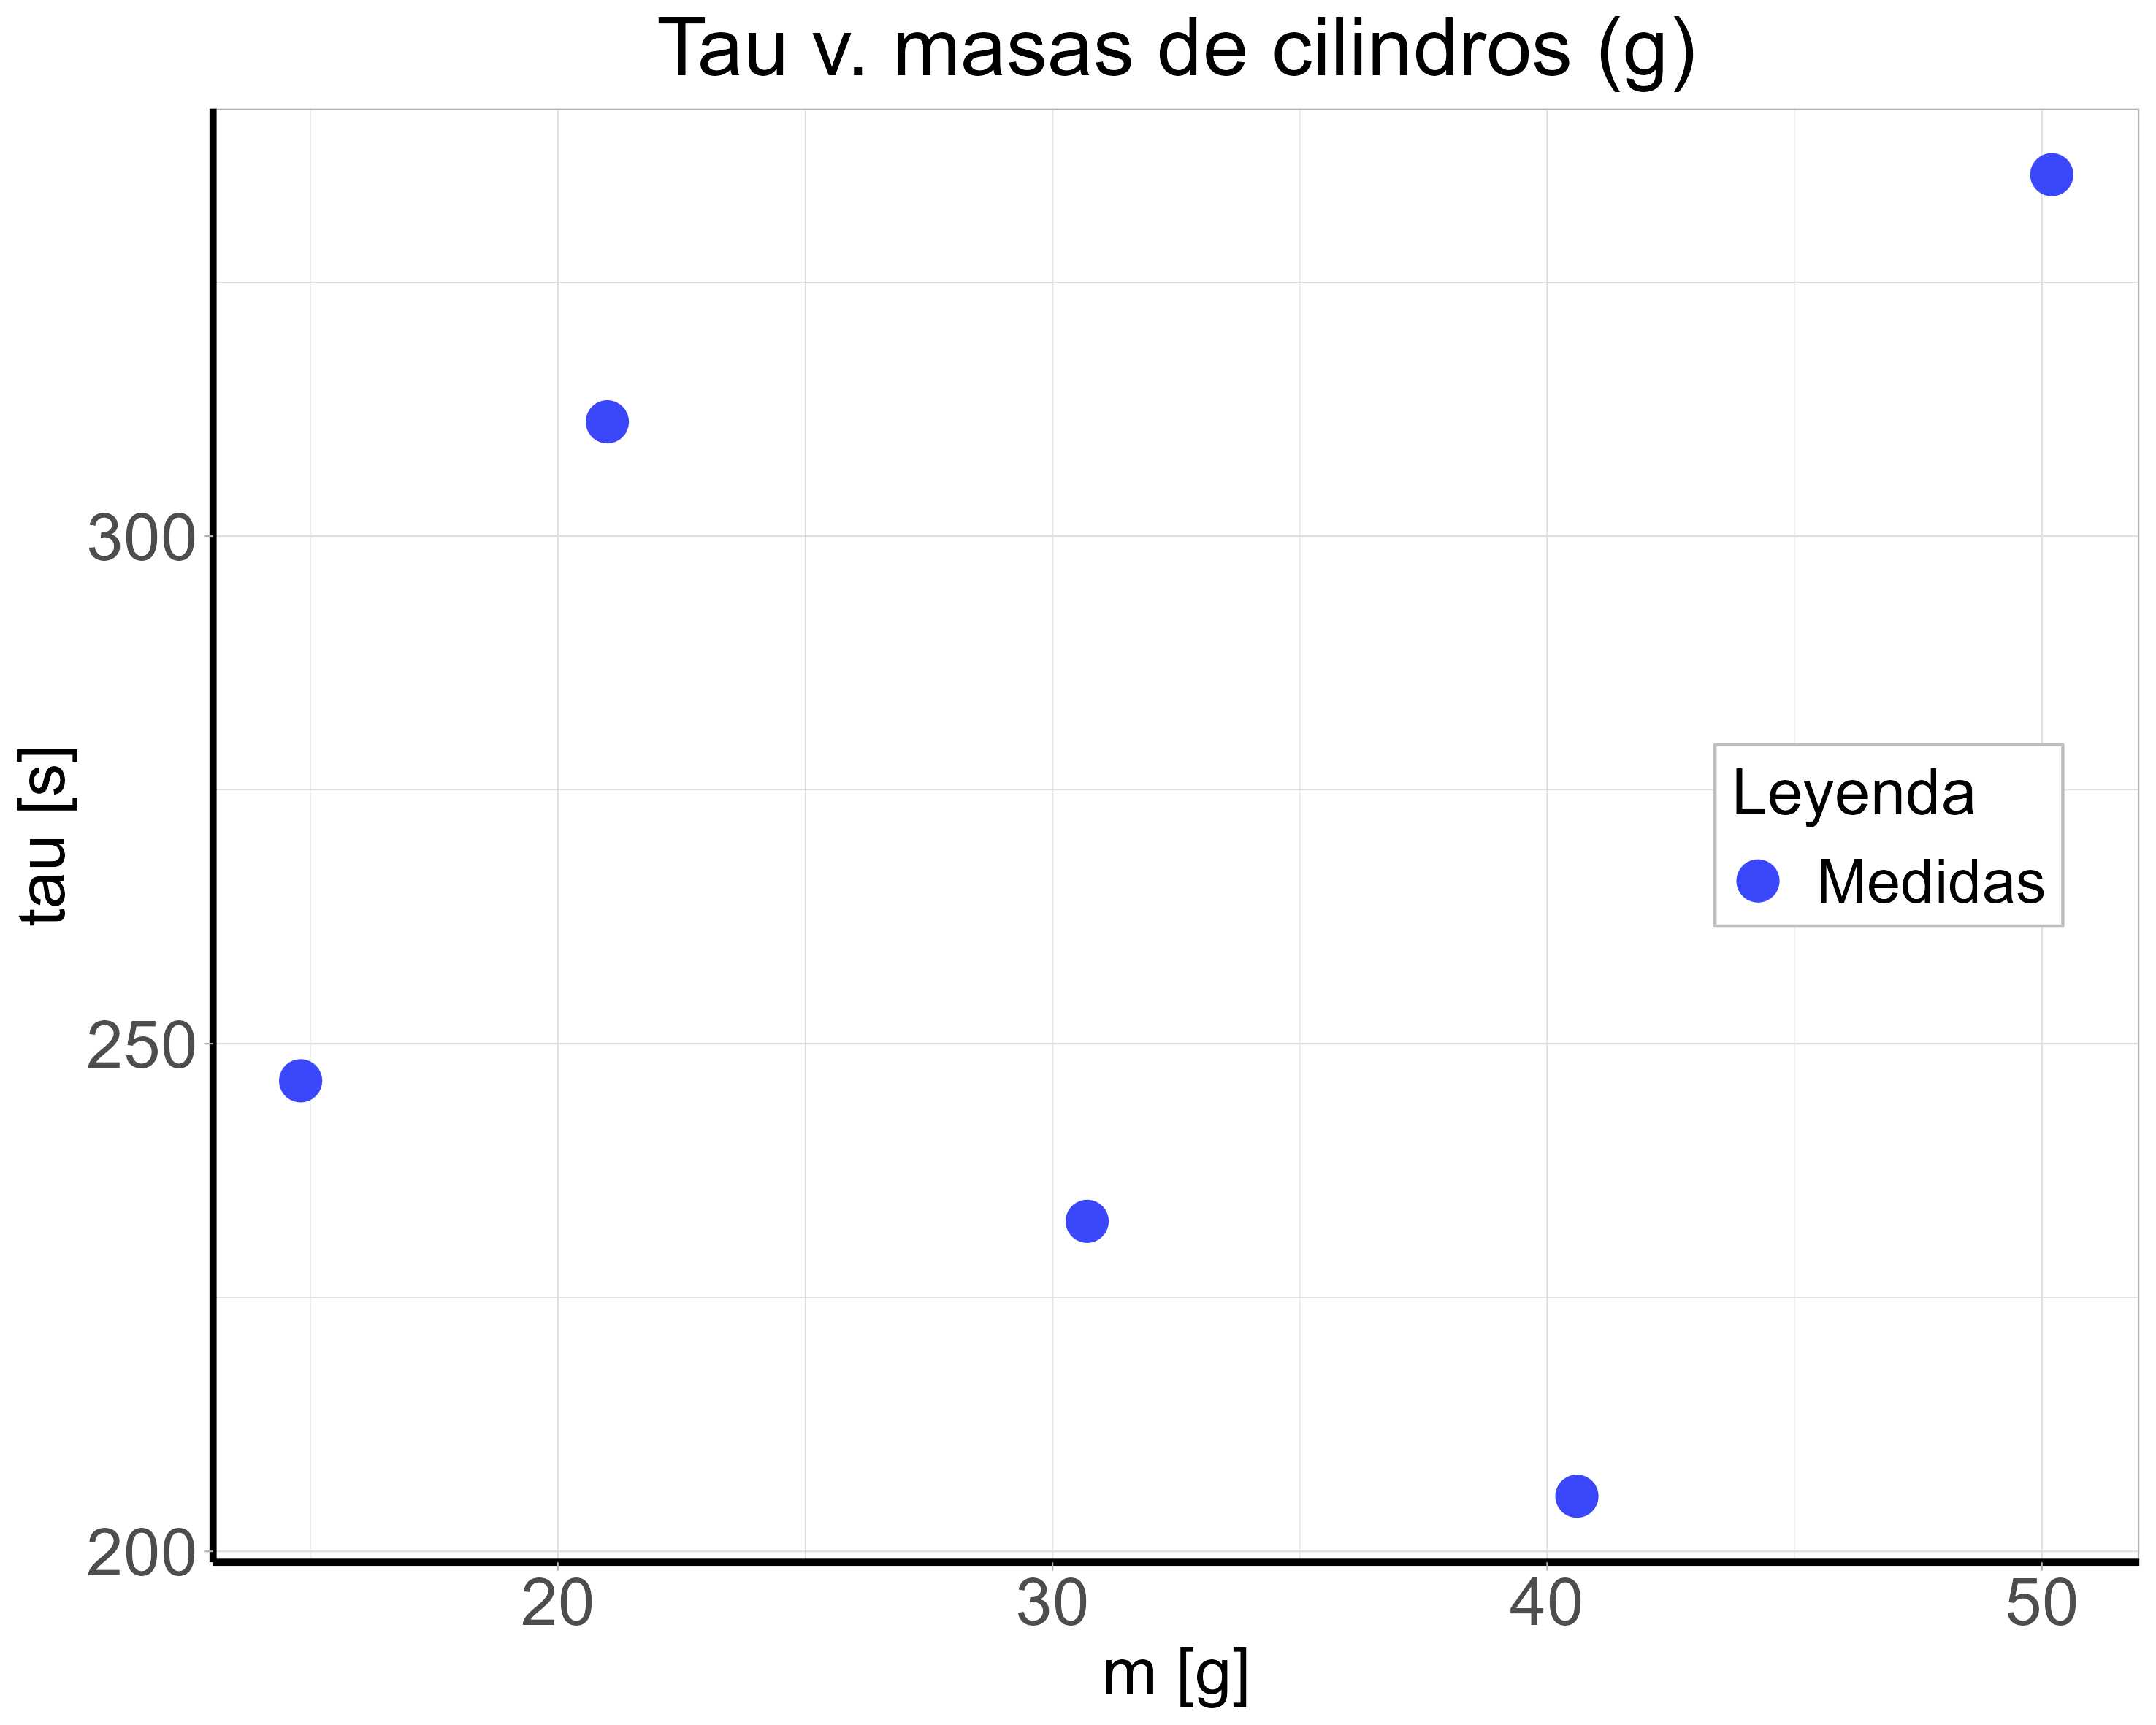
\includegraphics[height=5cm]{media/TauvM.png}
        \caption{Segunda medición}
    \end{subfigure}
    \caption{Aumento de la temperatura en el tiempo dentro del calorímetro.}
    \label{fig:electemp}
\end{figure}

No se evidencia ninguna relación entre la masa y el área superficial con el coeficiente.


\subsection{Calentamiento}


\section{Conclusiones}


\begin{thebibliography}{X}

\bibitem{pasco} Instruction Manual and Experiment Guide for the PASCO scientific Model TD-8551A. \path{https://cdn.pasco.com/product_document/Mechanical-Equivalent-of-Heat-Apparatus-Manual-TD-8551A.pdf}

\bibitem{purcell} Edward M. Purcell, David J. Morin. Electricity and Magnetism (2013).

\bibitem{scehu} Curso Interactivo de Física en Internet. Calor específico de un sólido. \path{http://www.sc.ehu.es/sbweb/fisica3/calor/calorimetro/calorimetro.html}. 

\bibitem{prof} Evelio, R. J.(2023). Ley de enfriamiento

\end{thebibliography}

\end{document}